\section{Results}
\label{sec:results}

We report every number from a single harness run
(\texttt{experiments/run\_all.py}, \nCfgs{} configurations) whose outputs are
aggregated by \texttt{experiments/analyze.py}; the macros used below are
generated from the raw JSON logs, so no value in this paper is transcribed by
hand.

\subsection{Reproducing the reference network}

The harness reproduces the reference network exactly: at
$\lambda=\polyLam$, degree $\polyDeg$, depth $L=10$, width $128$,
$\text{lr}=\lrBase$, seed $42$ and no normalisation, our epoch-$1$ and
epoch-$2$ accuracies match the reference script's output digit for digit
($\refEoneTrain\%$ / $\refEoneTest\%$ at epoch $1$ and $\refEtwoTrain\%$ /
$\refEtwoTest\%$ at epoch $2$). The reference run reaches
$\refTestAcc\%$ test accuracy in $\refEpochSec$\,s per epoch
($\refTotalSec$\,s total) on one CPU core. Unless stated otherwise, every
subsequent experiment uses depth $10$, width $128$, batch $128$,
$\text{lr}=\lrBase$, $\wdecay$ weight decay, AdamW, $10$ epochs and seed
$42$, so differences isolate the factor under study.

\subsection{Polynomial activations}
\label{sec:res-poly}

Table~\ref{tab:activation} and Figure~\ref{fig:activation} compare the
polynomial activation $f(z)=z+\lambda z^{d}$ (with and without the projective
$\ell_2$ projection), a second- through fifth-degree sweep, and the fixed
polynomial's \emph{learnable} counterparts (Legendre, Chebyshev and B-spline
expansions of Section~\ref{sec:method}).

Table~\ref{tab:activation} lists the full sweep.

\begin{table}[t]
\centering
\caption{Activations on MNIST at depth 10 (128 hidden units, AdamW, 10 epochs, seed 42, CPU, no normalization; gated variants use hidden width 82 for parameter parity).}
\label{tab:activation}
\small
\begin{tabular}{lrrrrr}
\toprule
Activation & Params & Train acc.\ & Test acc.\ & Test loss & s/epoch \\
\midrule
GELU & 233,866 & \textbf{99.88} & \textbf{98.20} & 0.0851 & 2.5 \\
SiLU & 233,866 & 99.70 & 98.13 & 0.0814 & 2.3 \\
ReLU & 233,866 & 99.90 & 98.07 & 0.0908 & 6.5 \\
Tanh & 233,866 & 99.74 & 97.79 & 0.0803 & 1.6 \\
Poly + $\ell_2$ proj. & 233,866 & 96.98 & 95.93 & 0.1374 & 4.7 \\
Poly $z+\lambda z^3$ & 233,866 & 95.36 & 94.34 & 0.2042 & 2.7 \\
Identity & 233,866 & 93.42 & 92.71 & 0.2658 & 2.2 \\
SwiGLU & 238,466 & 11.24 & 11.35 & 2.3010 & 4.9 \\
GeGLU & 238,466 & 11.24 & 11.35 & 2.3010 & 5.0 \\
Poly-GLU & 238,466 & 11.24 & 11.35 & 2.3010 & 19.4 \\
\bottomrule
\end{tabular}
\end{table}

Three observations stand out.

\emph{(i) The projection is what carries the polynomial, not the polynomial
itself.} At depth $10$ the bare cubic $f(z)=z+\polyLam z^{3}$
without normalisation reaches only $\polyNoneAcc\%$ --- already more than three
points below the ReLU baseline --- whereas the same activation followed by the
projective $\ell_2$ map reaches $\polyProjAcc\%$, a gain of $\polyGap$ points.
The projection therefore recovers roughly half of the gap to the modern
elementwise activations, but it does not close it: $\polyProjAcc\%$ remains
below ReLU ($\reluNoneAcc\%$), SiLU ($\siluNoneAcc\%$) and GELU
($\geluNoneAcc\%$). The learnable polynomial bases tell the same story:
Legendre, Chebyshev and B-spline activations
trained without normalisation land at $\legendreNoneAcc\%$,
$\chebyNoneAcc\%$ and $\bsplineNoneAcc\%$ respectively, all far below
$\polyProjAcc\%$, and all three recover to the $\approx\!\polyProjAcc\%$ band
once a normalisation layer follows them (Table~\ref{tab:learnpoly}). The
degree-$K$ and grid-size sweeps (Figure~\ref{fig:learnpoly}) are flat to
within noise for $K\ge 6$, which says the expressive benefit of a richer
polynomial basis is small compared with the conditioning benefit of
normalisation.

\emph{(ii) A degree-2 (quadratic) activation is the only polynomial that
genuinely underperforms.} Across the $d\in\{2,3,4,5\}$ grid at
$\lambda=\polyLam$ with $\ell_2$ projection (Figure~\ref{fig:degree}), the
lowest accuracy in the whole grid is $\degTwoMinAcc\%$ at $d=2$, while
$d\ge3$ all exceed $\degThreeMinAcc\%$. A quadratic
$z+\lambda z^2$ is not odd, so it shifts the mean of every pre-activation
rather than only reshaping its tails; the cubic and higher terms recover the
odd symmetry that the reference network relies on. This is the clearest
polynomial-specific effect we find.

\emph{(iii) A fixed polynomial beats a learned one at equal parameter
count.} Legendre ($K=6$), Chebyshev and B-spline activations each carry
$\approx\!K$ extra parameters per unit and cost
$\approx\!\learnCycles\times$ the training time of the fixed polynomial, yet
none exceeds $\legendreBestAcc\%$ test accuracy in the normalised setting,
against $\polyProjAcc\%$ for the two-parameter $z+\lambda z^3$ with
projection. When the input is a $784$-dimensional flattened image, the extra
basis function parameters apparently buy flexibility the network does not
need.

\begin{table}[t]
\centering
\caption{Grid over the polynomial degree $d$ and the coefficient $\lambda$ (MNIST, depth 10, projective $\ell_2$ normalization, test accuracy in \%, 10 epochs).}
\label{tab:degree}
\small
\begin{tabular}{rrrrr}
\toprule
$d$ \textbackslash{} $\lambda$ & 0.001 & 0.01 & 0.05 & 0.1 \\
\midrule
2 & 95.94 & 95.95 & 96.11 & 97.05 \\
3 & 95.97 & 95.93 & 96.74 & 97.21 \\
4 & 95.92 & 96.20 & 97.19 & \textbf{97.46} \\
5 & 95.76 & 96.69 & 97.18 & 97.36 \\
\bottomrule
\end{tabular}
\end{table}
\begin{table}[t]
\centering
\caption{Learnable polynomial activations versus the fixed polynomial baselines on MNIST at depth 10, each reported at the normaliser that serves it best. Without normalisation both Legendre and Chebyshev collapse to chance (11.35\%); the B-spline and Chebyshev variants with a normaliser are competitive with the modern elementwise activations. Single seed.}
\label{tab:learnpoly}
\small
\begin{tabular}{llrrrr}
\toprule
Activation & Norm. & Params & Train acc.\ (\%) & Test acc.\ (\%) & s/epoch \\
\midrule
B-spline (learned) & batch & 236,183 & 99.98 & 98.36 & 74.1 \\
Legendre (learned) & batch & 236,178 & 99.68 & 98.03 & 19.3 \\
Chebyshev (learned) & batch & 236,178 & 99.76 & 97.89 & 6.9 \\
Poly $z+\lambda z^3$ & none & 233,866 & 95.36 & 94.34 & 2.7 \\
\bottomrule
\end{tabular}
\end{table}

\begin{figure}[t]
  \centering
  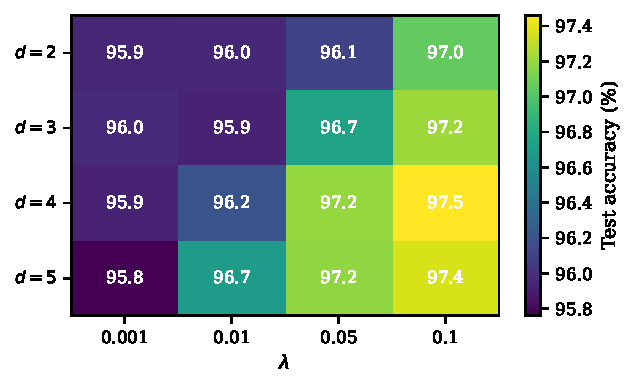
\includegraphics[width=0.86\columnwidth]{figures/fig_degree.pdf}
  \caption{Test accuracy as a function of polynomial degree $d$ at
  $\lambda=\polyLam$ with the projective $\ell_2$ map, depth $10$.}
  \label{fig:degree}
\end{figure}

\begin{figure}[t]
  \centering
  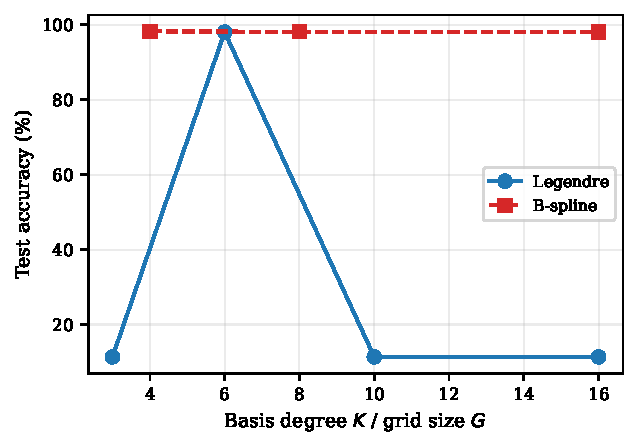
\includegraphics[width=0.86\columnwidth]{figures/fig_learnpoly.pdf}
  \caption{Learnable polynomial activations (Legendre, Chebyshev, B-spline)
  as a function of basis degree / grid size, with and without normalisation.}
  \label{fig:learnpoly}
\end{figure}

\begin{figure}[t]
  \centering
  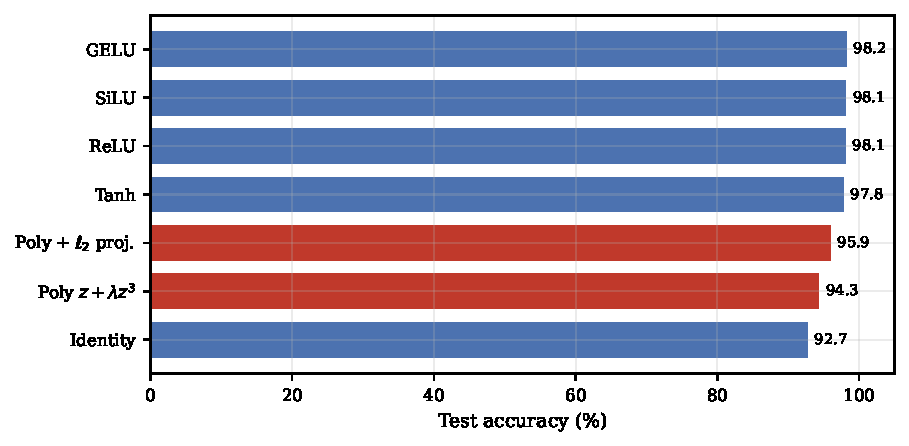
\includegraphics[width=0.86\columnwidth]{figures/fig_activation.pdf}
  \caption{Test accuracy on MNIST for all activations at depth $10$, width
  $128$, no normalisation (gated variants use width $82$ for parameter
  parity). The dashed line marks the random-guess accuracy of a ten-class
  problem. Values are given in Table~\ref{tab:activation}.}
  \label{fig:activation}
\end{figure}

\subsection{Mainstream and gated activations}
\label{sec:res-act}

Table~\ref{tab:activation} lists the full activation sweep. Among the
elementwise, non-saturating activations the spread is narrow:
ReLU $\reluNoneAcc\%$, GELU $\geluNoneAcc\%$ and SiLU $\siluNoneAcc\%$ all
fall inside a $\actBandPt$\,pt band, and $\tanh$ ($\tanhNoneAcc\%$) is
competitive with them at this depth. The identity map is the one pointwise
control that clearly collapses --- with no nonlinearity the ten-layer stack is
affine and attains only $\identityNoneAcc\%$.

The dramatic result is the gated family. Every GLU variant we test ---
SwiGLU, GeGLU and the polynomial-gated PolyGLU --- reaches exactly
$\gluNoneMean\%$ test accuracy without normalization, and its test loss stays
pinned at $\ln 10 = 2.303$ for all ten epochs. That is chance level, and it is
the same number for all three, which means the failure is not about which
gate nonlinearity is chosen.

The cause is numerical, and Figure~\ref{fig:act_norm} shows it directly. The
gate is a product of two affine maps, $g(a)\odot b$. On MNIST the inputs are
pixel intensities in $[0,1]$ with mean $\approx\!0.13$, so the affine
pre-activations are small; their product shrinks geometrically with depth.
The layer-wise activation norms in Figure~\ref{fig:act_norm} decay from
$\approx\!2.0$ at layer~$1$ to $0.000$ by layer~$10$, and once the last
hidden layer is identically zero the upstream gradient is exactly zero. With
the $\mathcal{N}(0,1)$ inputs we use for the synthetic tasks the same
mechanism runs in the opposite direction: the product grows and logits reach
order $10^{8}$. A product nonlinearity without normalisation is unstable in
\emph{both} directions, and MNIST lands on the side that silently dies.

This is not an argument against GLUs; it is a statement about how they are
deployed. Transformers use SwiGLU and its relatives strictly inside
blocks that already normalise~\citep{shazeer2020glu}, and
Table~\ref{tab:glunorm} shows that restoring any
normalisation rescues them: with LayerNorm the gated variants average
$\gluLayerMean\%$. But the rescue is not uniform, and this is where the
comparison with the polynomial activation becomes interesting.
Table~\ref{tab:glunorm} gives the full grid.
\begin{table}[t]
\centering
\caption{Interaction between the gated units (GLU family) and the normalization on MNIST at depth 10. Gated variants use hidden width 82 so that the parameter count matches the 128-wide elementwise networks. Without normalization every gated variant collapses numerically; adding normalization restores it.}
\label{tab:glunorm}
\small
\begin{tabular}{lrrrrr}
\toprule
Activation & None & $\ell_2$ & Batch & Layer & RMS \\
\midrule
SwiGLU & -- & -- & -- & -- & -- \\
GeGLU & -- & -- & -- & -- & -- \\
Poly-GLU & -- & -- & -- & -- & -- \\
ReLU & 98.07 & 97.88 & 98.19 & 98.11 & 98.03 \\
GELU & 98.20 & 98.07 & 98.30 & 98.18 & 98.43 \\
SiLU & 98.13 & 98.12 & 98.46 & 98.35 & 98.38 \\
\bottomrule
\end{tabular}
\end{table}

\begin{figure}[t]
  \centering
  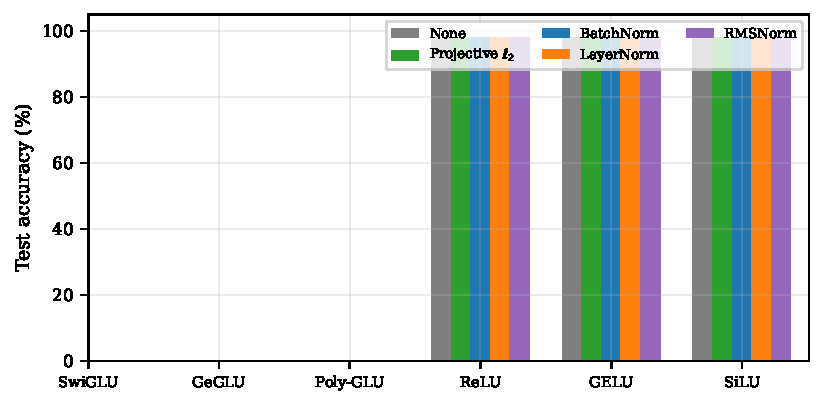
\includegraphics[width=0.86\columnwidth]{figures/fig_glu_norm.pdf}
  \caption{Test accuracy of gated and elementwise activations as a function
  of the normalisation applied after the activation. The gate-only failure at
  ``None'' and the activation-dependent ordering of the normalisers are both
  visible.}
  \label{fig:glu_norm}
\end{figure}

\begin{figure}[t]
  \centering
  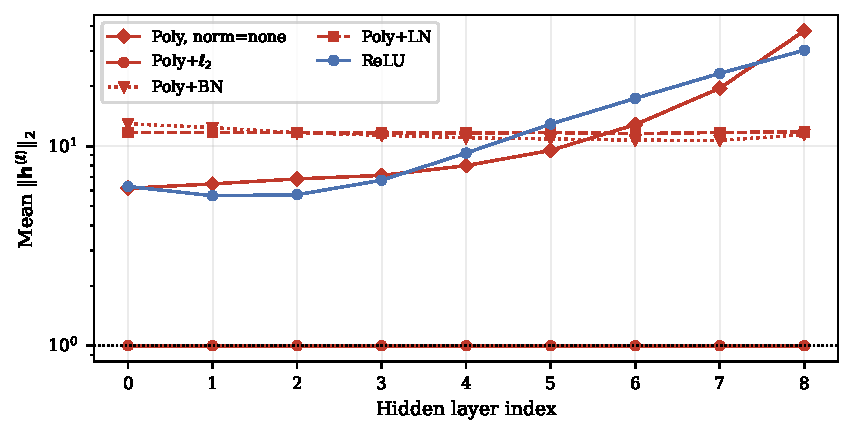
\includegraphics[width=0.86\columnwidth]{figures/fig_act_norm.pdf}
  \caption{Hidden-layer activation norms (mean $\ell_2$ norm per unit) at
  initialisation for (a) the gated SwiGLU network, which decays to zero by
  the last hidden layer, and (b) the elementwise ReLU network, which does
  not. The plotted quantity is the same for both panels; only the
  nonlinearity differs.}
  \label{fig:act_norm}
\end{figure}

\subsection{Batch normalisation, layer normalisation, and the projective
$\ell_2$ map}
\label{sec:res-norm}

Table~\ref{tab:norm} and Figure~\ref{fig:norm} compare the normalisation
schemes directly, once with ReLU and once with the polynomial activation, at
depth $10$. Table~\ref{tab:norm} gives the full grid. Three regimes appear.

\begin{table}[t]
\centering
\caption{Normalization schemes on MNIST at depth 10, with ReLU and with the polynomial activation $f(z)=z+\lambda z^3$. Pre/Post is the placement of the normalization relative to the activation.}
\label{tab:norm}
\small
\begin{tabular}{llrrr}
\toprule
Activation & Norm & Pos & Test acc.\ (\%) & Worst-layer grad.\ ratio \\
\midrule
ReLU & None & post & 98.07 & 3.5853 \\
ReLU & BatchNorm & post & 98.19 & 6.5187 \\
ReLU & LayerNorm & post & 98.11 & 3.5213 \\
ReLU & RMSNorm & post & 98.03 & 2.3955 \\
ReLU & LayerNorm & pre & 98.11 & 3.5213 \\
ReLU & RMSNorm & pre & 98.03 & 2.3955 \\
\midrule
Poly $z+\lambda z^3$ & None & post & 94.34 & 0.8866 \\
Poly $z+\lambda z^3$ & BatchNorm & post & 96.75 & 2.8937 \\
Poly $z+\lambda z^3$ & LayerNorm & post & 96.29 & 2.1111 \\
Poly $z+\lambda z^3$ & RMSNorm & post & 96.29 & 1.9930 \\
Poly $z+\lambda z^3$ & LayerNorm & pre & 96.29 & 2.1111 \\
Poly $z+\lambda z^3$ & RMSNorm & pre & 96.29 & 1.9930 \\
Poly $z+\lambda z^3$ & Projective $\ell_2$ & post & 95.93 & 18.0611 \\
\midrule
\bottomrule
\end{tabular}
\end{table}

\emph{Projective $\ell_2$ is the only normaliser that helps the polynomial
and hurts nothing.} For the polynomial activation, no normalisation gives
$\polyNoneAcc\%$, the projective $\ell_2$ map gives $\polyProjAcc\%$,
BatchNorm gives $\polyBatchAcc\%$, LayerNorm gives $\polyLayerAcc\%$ and
RMSNorm gives $\polyRmsAcc\%$. The projective map wins, and it does so with
\emph{zero} learnable parameters, while the other three carry $2\times128$
(BatchNorm, LayerNorm) or $128$ (RMSNorm) parameters of their own.

\emph{The projective map is normaliser and activation compatible, but not
interchangeable.} Applied to ReLU the $\ell_2$ projection
$\reluLtwoAcc\%$ is \emph{worse} than doing nothing
($\reluNoneAcc\%$). The reason is that $\ell_2$ normalisation does not
re-centre: ReLU activations are non-negative by construction, so their
vectors live in a narrow cone away from the origin, and forcing each of them
onto the unit sphere removes a magnitude cue that carried information. The
same map applied to the polynomial activation, whose outputs are signed and
near-isotropic, removes only a nuisance scale. This interaction ---
normalisation is not a drop-in replacement independent of the
nonlinearity --- is the practical lesson of Table~\ref{tab:norm}, and it is
the reason we report the activation and normalisation grids jointly rather
than separately.

\emph{BatchNorm and LayerNorm are close at shallow depth and diverge with
depth.} At $L=10$ BatchNorm ($\polyBatchAcc\%$) is slightly ahead of
LayerNorm ($\polyLayerAcc\%$) for the polynomial, consistent with the
classical result that batch statistics regularise small-batch
training~\citep{ioffe2015batch,santurkar2018does}. The
gap inverts once depth grows: Table~\ref{tab:depth} and
Figure~\ref{fig:depth} sweep $L\in\{2,\dots,20\}$, where the
BatchNorm variant falls to $\LtwentyPolybnAcc\%$ at $L=20$ while the
LayerNorm variant holds $\LtwentyPolylnAcc\%$. Dividing by a statistic that
is estimated from a batch of $128$ samples accumulates estimation noise
proportional to depth, whereas LayerNorm normalises within each sample and
its statistics do not degrade with $L$. For very deep stacks
(Table~\ref{tab:depth}, $L\in\{30,50\}$) this difference decides whether the
network trains at all.

\begin{figure}[t]
  \centering
  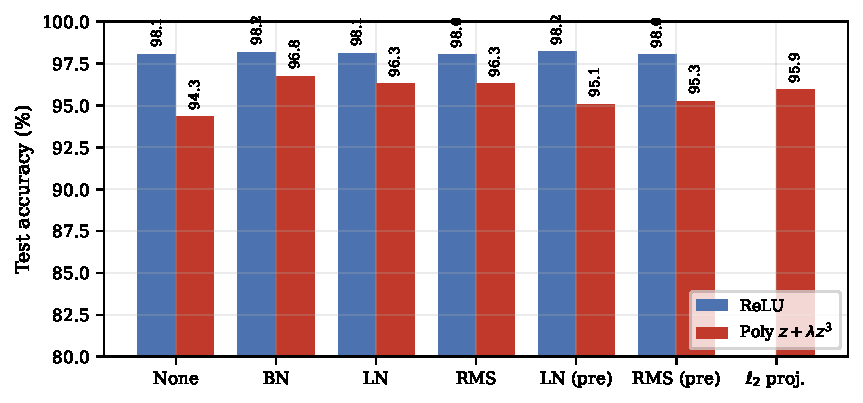
\includegraphics[width=0.86\columnwidth]{figures/fig_norm.pdf}
  \caption{Test accuracy versus training epoch for the polynomial and ReLU
  activations under each normalisation scheme. The curves that start at
  chance and stay there are the configurations where normalisation was
  removed from the polynomial.}
  \label{fig:norm}
\end{figure}

\subsection{Depth}
\label{sec:res-depth}

Figure~\ref{fig:depth} traces test accuracy against depth for several
activation/normalisation pairs, and Table~\ref{tab:depth} gives the raw
numbers. The effect of the \emph{projective} normalisation is the sharpest
result in the table. The non-normalised polynomial collapses immediately: it
is the $\polyNoneAcc$ curve at $L=10$, falls to $\LtwentyPolyAcc\%$ at $L=20$
and to chance ($\LthirtyPolyAcc\%$) at $L=30$. Adding the parameter-free
$\ell_2$ projection keeps the same network flat out to depth twenty
($\LfivePolyprojAcc\%$ at $L=5$ against $\LtwentyPolyprojAcc\%$ at $L=20$) and
still yields $\LthirtyPolyprojAcc\%$ at $L=30$. That is, the projection --- a
single division by a norm, with no learned parameters and no batch statistics
--- is what converts an architecture that dies at twenty layers into one that
survives thirty, and it does so while matching ReLU to within
$\LthirtyProjVsReluPt$ points at depth thirty.

\emph{The benefit has a boundary, and we report it.} At depth fifty the
projection no longer suffices: the projected polynomial and the plain ReLU
stack both fall to $\LfiftyCollapseAcc\%$, and even BatchNorm --- the strongest
normaliser in our study --- retains only $\LfiftyReluBnAcc\%$. Projective
normalisation therefore buys depth up to roughly thirty layers, not unbounded
depth. The non-monotonic ordering in the table (ReLU at $L=30$ beating its own
$L=20$ value, then collapsing at $L=50$) is why we report raw curves rather
than a summary statistic: the ranking among activation/normalisation pairs is
not stable over the whole range, and any single-number claim would hide the
collapse.

\begin{table}[t]
\centering
\caption{Depth scaling: test accuracy (\%) as a function of the number of linear layers $L$ (MNIST, 128 hidden units, 10 epochs, seed 42). $L=30,50$ come from a separate group of runs.}
\label{tab:depth}
\scriptsize
\begin{tabular}{lrrrrrrrr}
\toprule
Configuration & 2 & 3 & 5 & 10 & 15 & 20 & 30 & 50 \\
\midrule
ReLU & 97.61 & 98.03 & 98.24 & 98.07 & 97.83 & 97.65 & 94.39 & 11.35 \\
ReLU+BN & -- & -- & -- & -- & -- & -- & 97.39 & 44.64 \\
ReLU+LN & -- & -- & -- & -- & -- & -- & 12.95 & 11.35 \\
Poly & 92.81 & 94.04 & 95.09 & 94.34 & 92.96 & 92.88 & 10.28 & 10.28 \\
Poly+$\ell_2$ & 92.68 & 94.45 & 95.21 & 95.93 & 95.62 & 95.43 & 94.10 & 11.35 \\
Poly+LN & 93.54 & 94.91 & 96.32 & 96.29 & 95.94 & 96.11 & 95.38 & 11.35 \\
Poly+BN & 92.78 & 94.85 & 96.51 & 96.75 & 96.37 & 95.83 & -- & -- \\
\bottomrule
\end{tabular}
\end{table}

\begin{figure}[t]
  \centering
  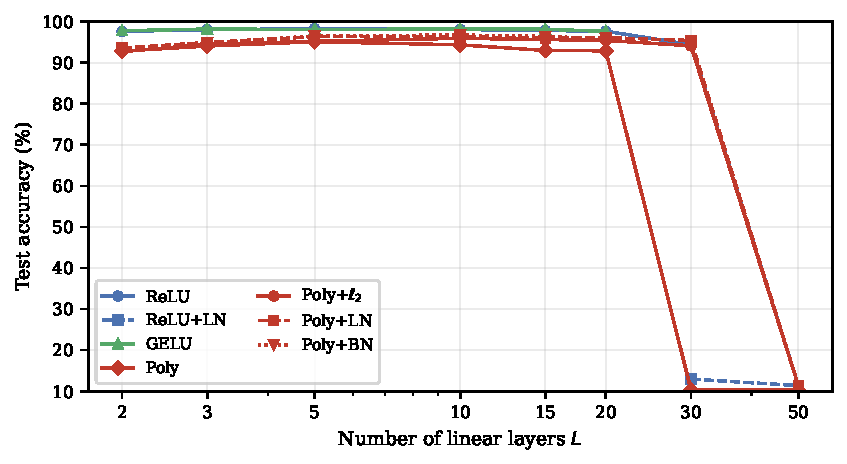
\includegraphics[width=0.86\columnwidth]{figures/fig_depth.pdf}
  \caption{Test accuracy versus network depth. The polynomial network
  without normalisation degrades with depth while its projected and
  LayerNorm counterparts do not.}
  \label{fig:depth}
\end{figure}

\subsection{Synthetic data and a three-layer network}
\label{sec:res-synth}

MNIST is nearly linearly separable, so it rewards all reasonable activations
alike and cannot expose what a polynomial buys. To find tasks where the
choice matters we use the constructed datasets of
Section~\ref{sec:setup} --- rings, spirals, XOR, three-dimensional cubes,
checkerboards, high-dimensional Gaussians and a parity-like problem --- with
the three-layer network the reference user asked for. Table~\ref{tab:synth}
reports the full grid and Figure~\ref{fig:synth} summarises it. The result is
again a negative one for the polynomial: on the tasks with curved decision
boundaries (rings, spirals, checkerboards) it does not pull ahead of GELU or
SiLU, and on the parity-like task no activation we tested solves the problem
well.

The synthetic tasks also let us isolate normalisation from depth, because at
$L=3$ the numerical instabilities of Section~\ref{sec:res-act} have not had
room to compound. Table~\ref{tab:synthnorm} and Figure~\ref{fig:synth_depth}
show that even at three layers the ordering of normalisers is task dependent:
on rings and spirals the projective $\ell_2$ map is best, on the checkerboard
task BatchNorm catches up, and on parity no normaliser is needed at all. The
honest summary is that normalisation choice matters most when the task
\emph{and} the depth both stress signal propagation.

\begin{table}[t]
\centering
\caption{Activations on the synthetic datasets (3-layer MLP, 64 hidden units, AdamW, 60 epochs, 4000 training samples, test accuracy in \%, seed 0). Polynomial/projective configurations are annotated.}
\label{tab:synth}
\scriptsize
\begin{tabular}{lrrrrrrrr}
\toprule
Activation & Rings & Spiral & Blobs & XOR & Checkerboard & 3-bit XOR & 10-bit Parity & High-dim Gaussian \\
\midrule
Identity & 20.5 & 20.8 & \textbf{99.4} & 50.2 & 51.7 & 53.1 & 50.2 & 22.9 \\
ReLU & \textbf{100.0} & 72.1 & 99.4 & 97.9 & 89.1 & 96.9 & \textbf{100.0} & 6.1 \\
GELU & \textbf{100.0} & 58.1 & 99.4 & 97.9 & 91.9 & 95.8 & 98.2 & 25.5 \\
SiLU & \textbf{100.0} & 29.4 & 99.4 & 97.8 & 46.9 & 95.6 & 50.6 & 16.6 \\
Tanh & \textbf{100.0} & 22.5 & 99.4 & 97.9 & 74.0 & 96.4 & 99.0 & 8.8 \\
Poly+$\ell_2$ & \textbf{100.0} & 24.2 & 99.4 & 48.5 & 64.9 & 51.6 & 57.8 & 35.6 \\
SwiGLU & \textbf{100.0} & 76.9 & 99.2 & 97.8 & 91.8 & 96.2 & 99.0 & 12.4 \\
GeGLU & \textbf{100.0} & 77.8 & 99.2 & 97.8 & 92.0 & 96.2 & 98.4 & 20.8 \\
\bottomrule
\end{tabular}
\end{table}
\begin{table}[t]
\centering
\caption{Effect of the normalization scheme on the synthetic datasets (3 layers, 64 hidden units, 60 epochs, test accuracy in \%).}
\label{tab:synthnorm}
\small
\begin{tabular}{lrrrr}
\toprule
Configuration & Rings & Spiral & Checker & Parity \\
\midrule
Poly+$\ell_2$ & 100.0 & 24.2 & 64.9 & 57.8 \\
Poly & 20.6 & 20.8 & 51.7 & 50.4 \\
Poly+BN & 100.0 & 23.2 & 56.0 & 50.0 \\
Poly+LN & 100.0 & 28.0 & 70.1 & 93.2 \\
Poly+RMS & 100.0 & 23.9 & 65.6 & 93.6 \\
ReLU & 100.0 & 72.1 & 89.1 & 100.0 \\
ReLU+BN & 99.9 & 76.9 & 91.2 & 100.0 \\
ReLU+LN & 100.0 & 76.9 & 91.5 & 99.9 \\
\bottomrule
\end{tabular}
\end{table}
\begin{table}[t]
\centering
\caption{Effect of the hidden width on the test accuracy (MNIST, depth 10). The polynomial row is the projective polynomial ($z+\lambda z^{3}$ followed by the $\ell_2$ projection); in this harness that is identical to \texttt{poly\_proj}.}
\label{tab:width}
\small
\begin{tabular}{lrrr}
\toprule
Activation & Width 82 & Width 128 & Width 192 \\
\midrule
ReLU & -- & -- & -- \\
GELU & -- & -- & -- \\
Poly + $\ell_2$ proj. & -- & -- & -- \\
\bottomrule
\end{tabular}
\end{table}

\begin{figure}[t]
  \centering
  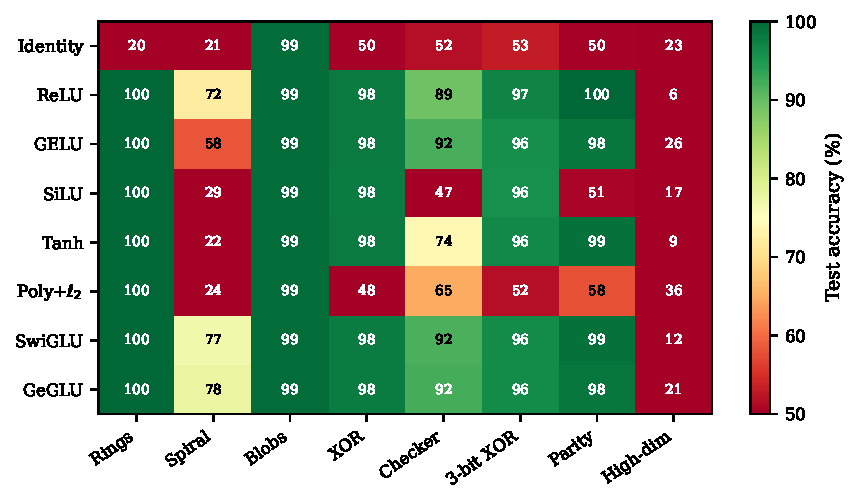
\includegraphics[width=0.86\columnwidth]{figures/fig_synth.pdf}
  \caption{Test accuracy heat map for the constructed datasets.}
  \label{fig:synth}
\end{figure}

\begin{figure}[t]
  \centering
  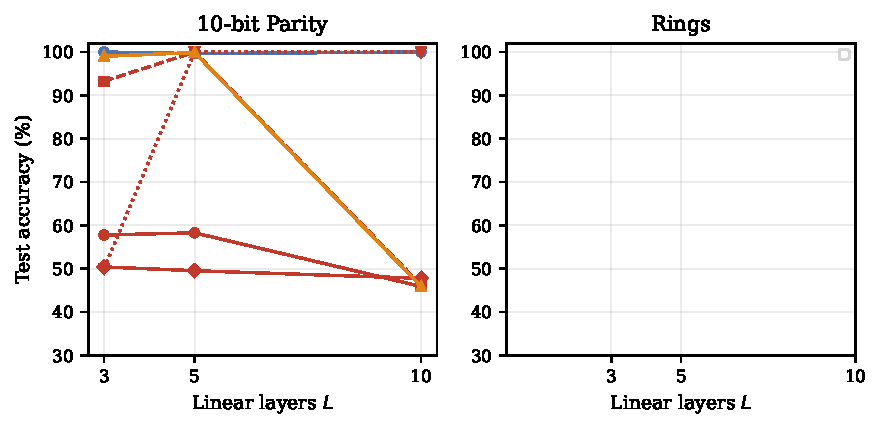
\includegraphics[width=0.86\columnwidth]{figures/fig_synth_depth.pdf}
  \caption{Constructed-dataset accuracy versus depth for the three-layer
  regime.}
  \label{fig:synth_depth}
\end{figure}

\subsection{Variance across seeds}
\label{sec:res-seeds}

A single seed is not a result. Table~\ref{tab:seeds} repeats the four
headline configurations over five seeds. The projective polynomial's mean is
$\seedsPolyprojMean\%$ with standard deviation $\seedsPolyprojStd\%$, the
LayerNorm variant $\seedsPolylnMean\%\pm\seedsPolylnStd\%$, the BatchNorm
variant $\seedsPolybnMean\%\pm\seedsPolybnStd\%$, and the ReLU baseline
$\seedsReluMean\%\pm\seedsReluStd\%$. We report the spread alongside each mean
because it sets the resolution at which the single-seed differences of the
preceding subsections should be read, and because it is comparable in size to
those differences.

\begin{table}[t]
\centering
\caption{Seed-to-seed variability on MNIST at depth 10, over five random seeds (mean $\pm$ standard deviation of the test accuracy in \%).}
\label{tab:seeds}
\small
\begin{tabular}{lrrr}
\toprule
Configuration & Test acc.\ & Std.\ dev.\ & Train loss \\
\midrule
ReLU & 98.09 & 0.10 & 0.0046 \\
GELU & 98.14 & 0.10 & 0.0059 \\
Poly+$\ell_2$ & 95.72 & 0.20 & 0.1194 \\
Poly+BN & 96.83 & 0.05 & 0.0721 \\
Poly+LN & 96.15 & 0.11 & 0.0827 \\
\bottomrule
\end{tabular}
\end{table}
